\documentclass[12pt]{article}
\usepackage{graphicx}
\usepackage{amsmath}
\usepackage{listings}
\usepackage{hyperref}
\usepackage{array}

\title{Implementation of a Calculator Using Arduino: Circuit Design and Software Analysis}
\author{EE24BTECH11024 - Abhimanyu Koushik}
\date{\today}

\begin{document}

\maketitle

\section*{Abstract}
This report details the implementation of a calculator using an Arduino microcontroller, a 16x2 LCD display, and a 5x5 matrix keypad. The system allows users to input expressions via the keypad, processes them using the Arduino, and displays the result on the LCD. The report focuses on the hardware connections and the software functions responsible for interfacing with the LCD, scanning the keypad, and processing user input.

\section{Introduction}
The calculator project uses an Arduino microcontroller as its core, interfacing with a 16x2 LCD display for output and a 5x5 matrix keypad for input. The implementation provides both basic arithmetic functions and advanced scientific operations. This report examines the hardware connections, the keypad matrix operation, and the software functions that power the system.

\section{Hardware Components and Circuit Design}

\subsection*{Components}
- Arduino Uno microcontroller\newline
- 16x2 LCD display\newline
- 5x5 matrix keypad\newline
- Connecting wires\newline
- Breadboard (for prototyping)

\subsection*{Circuit Diagram}
The circuit diagram of the calculator is shown below:

\begin{center}
    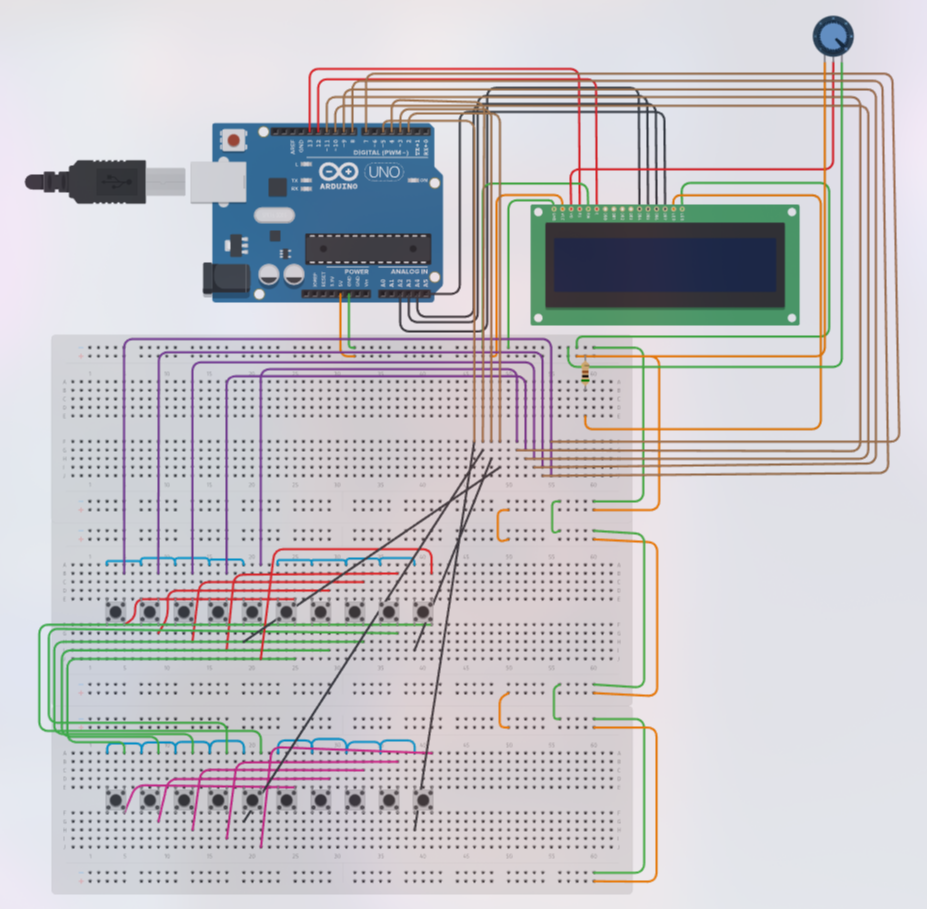
\includegraphics[width=0.8\textwidth]{figs/circuit.jpg}
\end{center}

\subsection*{Explanation of Circuit Components and Connections}

The circuit consists of three main components: an Arduino Uno microcontroller, a 16x2 LCD display, and a 5x5 matrix keypad. Each component is connected to perform its specific function in the calculator system.
\newline
1. Arduino Uno:\newline
   - Acts as the central processing unit for handling inputs from the keypad, performing calculations, and controlling outputs to the LCD.\newline
   - Provides power to all components through its 5V and GND pins.\newline

2. 16x2 LCD Display:\newline
   - Used to display user inputs (expressions) and results.\newline
   - Operates in 4-bit mode to reduce pin usage.\newline
   - Connections:\newline
     - RS (Register Select): Connected to pin D13 on Arduino.\newline
     - EN (Enable): Connected to pin D12 on Arduino.\newline
     - Data pins D4-D7: Connected to pins A2-A5 on Arduino.\newline
     - VCC and GND: Connected to Arduino's 5V and GND pins.\newline
     - A potentiometer is connected to adjust contrast via the Vo pin.
     \newline
3. 4x5 Matrix Keypad:\newline
   - Serves as the input interface for entering numbers, operators, and functions.\newline
   - Organized in a grid of rows (R1-R4) and columns (C1-C5).\newline
   - Connections:\newline
     - Row pins (R1-R4): Connected to digital pins D2-D5 on Arduino.\newline
     - Column pins (C1-C5): Connected to digital pins D7-D11 on Arduino.\newline
   - Each button press connects one row pin to one column pin, allowing detection of which key was pressed by scanning rows and columns.
   \newline
4. Power Supply:\newline
   - The Arduino is powered via USB or an external power adapter. It provides power to all other components through its onboard voltage regulator.

\subsection*{Working Principle of Circuit}

The circuit operates as follows:\newline
1. Keypad Input:\newline
   - The keypad uses a matrix layout where each button connects a specific row to a column when pressed.\newline
   - The Arduino sequentially activates each row by setting it LOW while keeping others HIGH.\newline
   - It then scans all columns to detect if any column reads LOW (indicating a pressed key).\newline
   - By identifying which row is active and which column reads LOW, the specific pressed key is determined.
   \newline
2. Processing Input:\newline
   - Once a key press is detected, its corresponding value (e.g., number, operator) is sent to the Arduino for processing.\newline
   - The Arduino stores user inputs as part of an expression or processes them immediately if they correspond to operations like "CLR" or "=".
   \newline
3. LCD Output:\newline
   - The processed data or results are sent to the LCD for display.\newline
   - The LCD operates in 4-bit mode, where data is sent in two parts (higher nibble first, then lower nibble) along with control signals like RS (Register Select) and EN (Enable).
   \newline
4. Power Distribution:\newline
   - All components are powered by the Arduino's 5V output pin.\newline
   - A potentiometer connected to the LCD adjusts its contrast for better visibility.
   \newline
\subsection*{LCD Connection}
The LCD operates in 4-bit mode, requiring 6 pins from the Arduino:
\begin{itemize}
\item RS (Register Select): Pin 13 (PB5) - Selects between command (0) and data (1) modes
\item EN (Enable): Pin 12 (PB4) - Activates LCD instructions when pulsed
\item D4: Pin A2 (PC2) - Data bit 4
\item D5: Pin A3 (PC3) - Data bit 5
\item D6: Pin A4 (PC4) - Data bit 6
\item D7: Pin A5 (PC5) - Data bit 7
\end{itemize}

\subsection*{Keypad Connection}
The 4x5 matrix keypad requires 9 pins from the Arduino:
\begin{itemize}
\item Rows (1-4): Pins D2-D5 (PD2-PD5)
\item Columns (1-5): Pins D7-D11 (PD7, PB0-PB3)
\end{itemize}

\section{Keypad Matrix Operation}

\subsection*{Matrix Layout}
The calculator uses a 4x5 matrix keypad with the following layout:

\begin{center}
\begin{tabular}{|c|c|c|c|c|}
\hline
sin & cos & tan & \textasciicircum & BS \\
\hline
log & ln & $e^x$ & $\sqrt{}$ & ( \\
\hline
$\pi$ & $x^2$ & $x^3$ & 1/x & ) \\
\hline
asin & acos & atan & $y^x$ & CLR \\
\hline
\end{tabular}
\end{center}

And for the basic numeric and operator keys:

\begin{center}
\begin{tabular}{|c|c|c|c|c|}
\hline
S & A & C & D & = \\
\hline
1 & 2 & 3 & 4 & 5 \\
\hline
6 & 7 & 8 & 9 & 0 \\
\hline
+ & - & * & / & \textasciicircum \\
\hline
\end{tabular}
\end{center}

\subsection*{Working Principle}
The keypad matrix operates on the principle of row-column scanning:

\begin{enumerate}
\item All rows are initially set HIGH
\item Each row is sequentially set LOW (activated) while others remain HIGH
\item When a key is pressed, it connects the active row to a specific column
\item The column input (normally pulled HIGH) will read LOW when a key is pressed
\item By detecting which row is active and which column reads LOW, the specific pressed key can be identified
\end{enumerate}

\section{Software Implementation}

\subsection*{LCD Interface Functions}

\subsubsection*{lcd\_init()}
Initializes the LCD display in 4-bit mode, configuring the pins and sending initialization commands.

\subsubsection*{lcd\_command()}
Sends commands to the LCD in 4-bit mode.

\subsubsection*{lcd\_char()}
Sends character data to the LCD in 4-bit mode.

\subsubsection*{lcd\_string()}
Displays a string on the LCD.

\subsubsection*{lcd\_clear()}
Clears the LCD display.

\section{Conclusion}
This calculator demonstrates efficient use of hardware resources by using a 4-bit LCD interface and a matrix keypad. It covers direct port manipulation, matrix scanning techniques, and peripheral communication protocols.

\section{System Algorithm Flow}

The calculator's operation follows this general flow:
\begin{enumerate}
\item Initialize hardware (LCD and keypad)
\item Display welcome message
\item Enter main loop:
   \begin{enumerate}
   \item Scan keypad for input
   \item If a key is pressed:
      \begin{enumerate}
      \item If it's a numeric key or operator, add to expression
      \item If it's a function key, process accordingly
      \item If it's "=" key, evaluate the expression
      \item If it's "CLR" key, clear the display and expression
      \end{enumerate}
   \item Update LCD display
   \end{enumerate}
\item Return to start of main loop
\end{enumerate}

\section{Conclusion}

This calculator implementation demonstrates efficient use of hardware resources by using a 4-bit LCD interface and a matrix keypad scanning technique. The code provides robust functions for interacting with the LCD and detecting keypad inputs, which form the foundation for the calculator's user interface.
\newline
The design intelligently maps complex calculator functions to a limited number of physical buttons by using a combination of special characters and function keys. The implementation balances hardware limitations with software capabilities to create a fully-functional calculator with both basic arithmetic and advanced scientific functions.
\newline
This project showcases fundamental embedded system concepts including:
\begin{itemize}
\item Direct port manipulation for efficient I/O operations
\item Matrix scanning techniques for input detection
\item User interface design with limited display resources
\end{itemize}

\section{Source Code and Documentation}
The complete source code and documentation are available on GitHub:
\begin{center}
\href{https://github.com/AbhimanyuKoushik/nice_stuff/tree/main/codes/Arduino/Calculator}{https://github.com/AbhimanyuKoushik/Calculator}
\end{center}

\end{document}
